%! Author = magnus.silverdal
%! Date = 2020-12-03

% Preamble
\documentclass[11pt]{beamer}
\usetheme{Copenhagen}
% Packages
\usepackage{amsmath}
\usepackage{graphicx}
\usepackage[utf8]{inputenc}
\usepackage[T1]{fontenc}


\title{Repetition Mekanik}
\author{Magnus Silverdal}
\institute{NTI Gymnasiet}
\date{\today}
% Document
\begin{document}
    \frame{\titlepage}

    \begin{frame}
        \frametitle{Begrepp}
        \begin{itemize}
            \item Positionen $s$ beskriver hur långt vi är från utgångspunkten. Vi kan själva välja var vi lägger noll-punkten
            men ofta används utgångspunkten som 0.
            \item Medelhastigheten $v_m$ är den genomsnittliga hastigheten under ett tidsintervall och den beräknas med
            $v_m=\frac{\Delta s}{\Delta t}$
            \item Momentanhastighet $v$ är hastigheten vid en given tid. Hastighet syftar alltid på momentanhastigheten.
            Kom ihåg att hastighet är en vektor, den har både storlek och riktning.
            \item Medelaccelerationen $a_m$ är den genomsnittliga accelerationen under ett tidsintervall och den beräknas med
            $a_m=\frac{\Delta v}{\Delta t}$
            \item Momentanacceleration $a$ är hastigheten vid en given tid. Acceleration syftar alltid på momentanaccelerationen.
            Kom ihåg att acceleration är en vektor, den har både storlek och riktning.
            \item Fritt fall är när något faller fritt utan luftmotstånd. Gravitationen ger då en konstant acceleration,
            tyngdaccelerationen $g$, som här i Sverige är $9.82 \frac{m}{s^2}$.
        \end{itemize}
    \end{frame}
    \begin{frame}
        \frametitle{s-t Diagram}
        \begin{figure}[!h]
            \includegraphics[width=\textwidth]{../images/chapter3/DistTime}
            \caption{Sträcka-tid diagram. Källa: Impuls Fysik 1}
        \end{figure}
    \end{frame}

        \begin{frame}
            \frametitle{v-t-diagram}

        \begin{figure}[!h]
            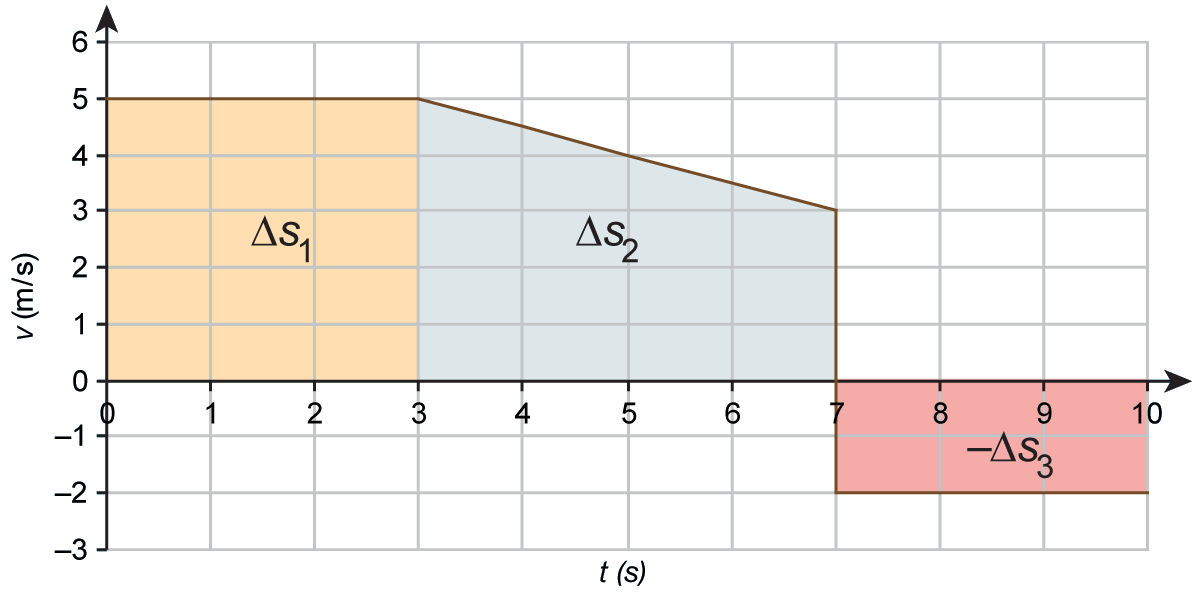
\includegraphics[width=\textwidth]{../images/chapter3/velocityTime.png}
            \caption{Hastighet-tid diagram. Källa: Impuls Fysik 1}
        \end{figure}
        Accelerationen är lutningen på kurvan, sträckan är arean under grafen. Observera att negativ sträcka betyder att
        föremålet rör sig tillbaka mot noll-punkten.
            \end{frame}
    \begin{frame}
        \frametitle{v-t-diagram}

        \begin{figure}[!h]
            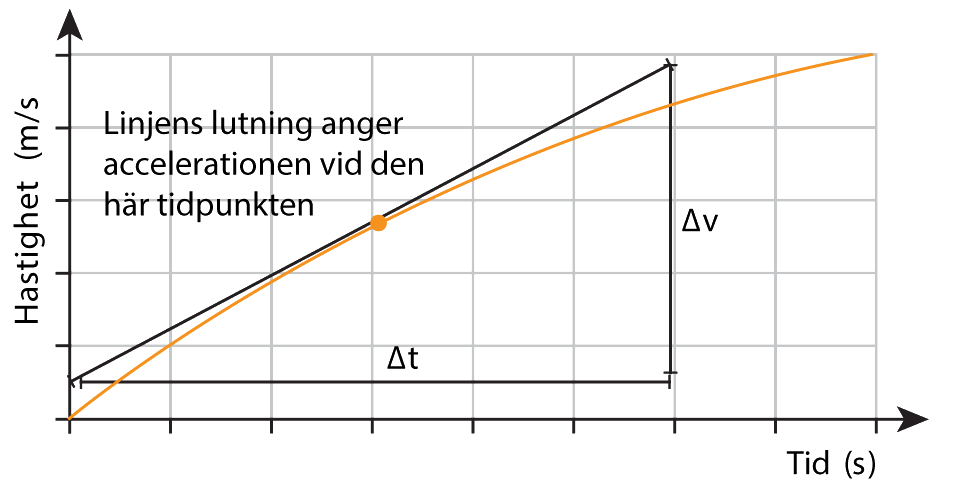
\includegraphics[width=0.5\textwidth]{../images/chapter3/velocityTimeAcceleration.png}
            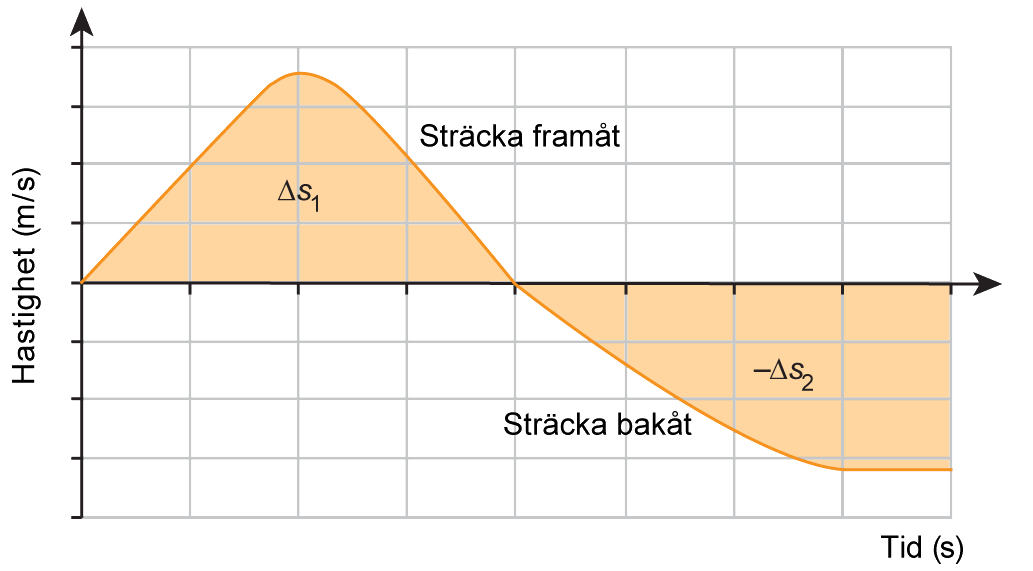
\includegraphics[width=0.5\textwidth]{../images/chapter3/velocityTimeDist.png}
            \caption{Hastighet-tid diagram. Källa: Impuls Fysik 1}
        \end{figure}
        \end{frame}
    \begin{frame}
        \frametitle{Acceleration-tid-diagram}


        \begin{figure}[!h]
            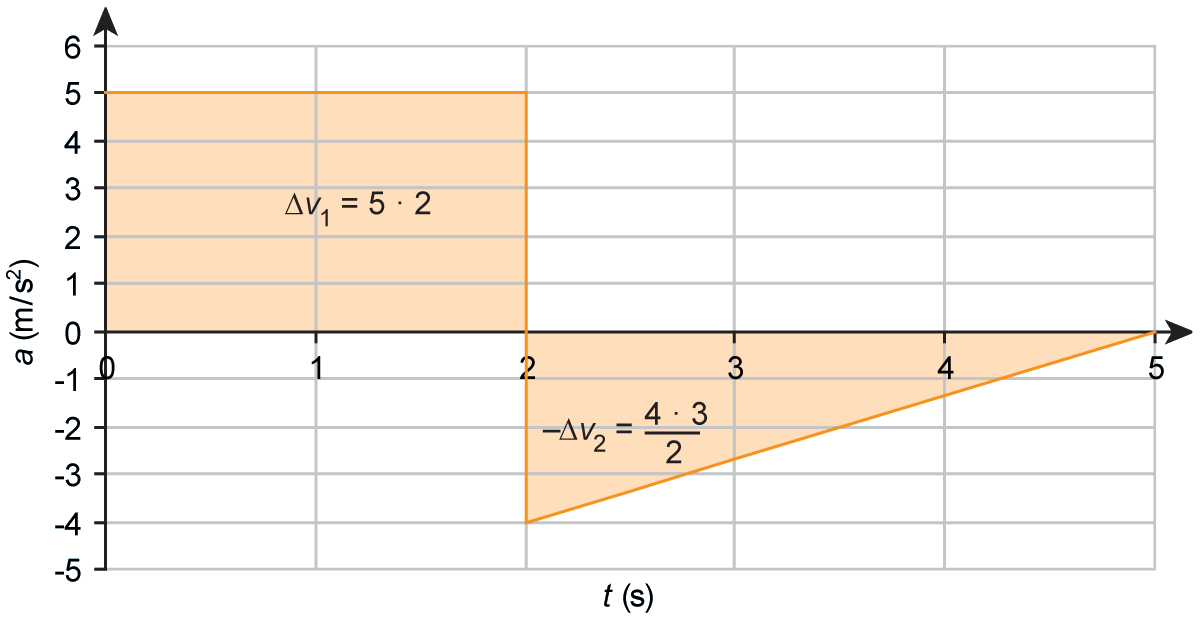
\includegraphics[width=\textwidth]{../images/chapter3/accelerationTime.png}
            \caption{Acceleration-tid diagram. Källa: Impuls Fysik 1}
        \end{figure}
        Förändringen av hastighet är arean under grafen.


    \end{frame}
    \begin{frame}
        \frametitle{viktiga samband}
        Vid konstant acceleration (till exempel fritt fall) gäller
        \begin{eqnarray}
            v&=&v_0+at \\
            s&=&v_0 t +  \frac{at^2}{2}
        \end{eqnarray}
    \end{frame}

    \begin{frame}
        \frametitle{Kraft}
        Krafter är vektorer som kan adderas.
        De har både storlek och riktning.
        \begin{itemize}
            \item Newtons 1:a lag: \\
            Om den resulterande kraften på ett föremål är noll, så befinner sig föremålet antingen i vila eller så rör det sig med konstant hastighet utefter en rät linje.
            \item Newtons 2:a lag:
            \begin{equation}
                F=m a
            \end{equation}
            Om den resulterande kraften $F_R$ på ett föremål med massan $m$ inte är noll, så kommer föremålet att accelerera med accelerationen $a$.
            \item Newtons 3:e lag \\
            Om föremålet A påverkar föremålet B med en kraft, så påverkar B föremålet A med en lika stor men motriktad kraft. Dessa krafter verkar utefter samma linje.
        \end{itemize}
    \end{frame}
    \begin{frame}
        \frametitle{Några krafter}
        Gravitationskraft
        \begin{equation}
            F=G \frac{m_1 m_2}{r^2}
        \end{equation}
        Tyngdkraft
        \begin{equation}
            F=m g
        \end{equation}
        Fjäderkraft
        \begin{equation}
            F=k \Delta l
        \end{equation}
        Friktionskraft
        \begin{equation}
            F=\mu F_N
        \end{equation}


    \end{frame}

        \begin{frame}
        \frametitle{Arbete}
        Inom mekanik (läran om saker som rör sig) behövs en kraft $F$ för att förändra hur föremålen rör sig, enligt Newtons andra lag.
        Om det sker en förändring har ett arbete $W$ utförts och det definieras som
        \begin{equation}
            W = F \cdot s
        \end{equation}
        där $s$ är sträckan som kraften verkat längs. Arbetets enhet blir $Nm$

        \vspace{10}
        Detta gäller endast om kraften är konstant, det generella uttrycket är
        \begin{equation}
            W = \int F(s) ds
        \end{equation}

    \end{frame}

    \begin{frame}
        \frametitle{Energi}
        Arbete är en förändring av energin hos ett föremål. Inom Mekaniken betyder det att när en kraft förändrar
        föremålets rörelse så förändras föremålets energi. Eftersom energi inte kan skapas eller förstöras är arbete
        ett sätt att flytta energi från en form eller plats till en annan
        \begin{equation}
            W = \Delta E
        \end{equation}
        Detta gäller för det eller de föremål som studeras. Enheten för energi är Joule och betecknas $J$ men enligt
        formeln syns att det är exakt samma sak som $Nm$
    \end{frame}

    \begin{frame}
        \frametitle{Mekanisk energi}
        De energier som är relevanta i ett mekaniskt system är rörelseenergi, eller kinetisk energi
        \begin{equation}
            E_k = \frac{mv^2}{2}
        \end{equation}
        och lägesenergi eller potentiell energi
        \begin{equation}
            E_p = mgh
        \end{equation}
        All energi är relativ någon 0-nivå så när vi jämför energier måste vi tänka på att de ska ha samma nollnivå.
        I praktiken innebär det att höjd och hastighet ska mätas på samma relativa sätt.
    \end{frame}
    \begin{frame}
        \frametitle{Effekt och verkningsgrad}
        För att kunna jämföra och räkna på olika arbeten räcker det inte alltid att veta slutresultatet, det kan också
        spela roll hur lång tid arbetet tagit. Ett mått på detta är effekt. Definitionen på effekt är energiändring per tidsenhet
        \begin{equation}
            P = \frac{\Delta E}{\Delta t}
        \end{equation}
        För att beskriva hur stor del av den energi som behövs för ett arbete jämfört med hur mycket arbete som utförs
        används begreppet verkningsgrad.  Det är kvoten mellan de nyttiga, utförda arbetet och den tillförda energin.
        Eftersom effekten är arbete per tidsenehet och arbetet utförs under en given tid kan detta också skrivas som
        \begin{equation}
            \eta = \frac{E_{nyttig}}{E_{tillförd}} = \frac{P_{nyttig}}{P_{tillförd}}
        \end{equation}

    \end{frame}
    \begin{frame}
        \frametitle{Rörelsemängd}
        Rörelsemängd definieras som $ p = m v$ och det var den som Newton utgick ifrån när han härledde sina lagar\\
        Rörelsemängd överförs i form av en impuls vid kollisioner
        \begin{equation}
            F \Delta t = mv_e - m v_f
        \end{equation}
        där $v_f$ är hastigheten före och $v_e$ är hastigheten efter kollision
    \end{frame}
    \begin{frame}
        \frametitle{Kollisioner}
        Vi kollisioner mellan 2 föremål A och B bevaras rörelsemängden
        \begin{equation}
            p_{Af} + p_{Bf} = p_{Ae} + p_{Be}
        \end{equation}
        Om rörelseenergin också bevaras är kollisionen fullständigt elastisk

    \end{frame}
\end{document}